\documentclass{beamer}

\usepackage{graphicx}
\usepackage{hyperref}
\usepackage[latin1]{inputenc}
\usepackage[T1]{fontenc}
\usepackage[english]{babel}
\usepackage{listings}
\usepackage{xcolor,mathrsfs,url}
\usepackage{amssymb}
\usepackage{amsmath}
\usepackage{ifthen}

% The command to define a subsection is '\subsec{}' and NOT '\subsection'.
% This code generates the bar. Don't edit.
\newcommand{\midbarnew}{}
\newcommand{\subsec}[1]
{
  \ifthenelse{\equal{#1}{}}
  {\renewcommand{\midbarnew}{} \subsection{}}
  {\renewcommand{\midbarnew}{ $\mid$ } \subsection{#1}}
}

% change the pictures here, if necessary. logobig and logosmall are the internal names
% for the pictures: do not modify them, just change "hulogo" and "logo". Pictures must be 
% supplied as JPEG, PNG or PDF
%########################################

\pgfdeclareimage[height=2cm]{logobig}{logo} % use hucase instead for the Humboldt-Case Logo
\pgfdeclareimage[height=1cm]{logosmall}{logo}

% use this number to modify the scaling of the headline on titlepage
\def\titlescale{1.0}


\def\authora{David Jinkins}	% First Author
\def\affa{Department of Economics-CBS} % First Author's Affiliation
\def\authorb{}  % Second Author
\def\affb{} % Second Author's Affiliation
\def\authorc{}  % Third Author
\def\affc{} % Third Author's Affiliation
\def\linka{}	% Link to your institution's/ personal website
\def\linkb{}
\def\linkc{}\def\email{\href{mailto:bs.eco@cbs.dk}{bs.eco@cbs.dk}}	% Your email address

\title[ National Accounting and Exchange Rates.]{International Economics - B.Sc. IB\\ 8. Open-Economy Macroeconomics: \\ National Accounting and Balance of Payment. Exchange Rates \\  \footnotesize{May $1^{st}$, 2014}}
\institute{Economics Department CBS}
%Start of the document
\begin{document}


\frame[plain]{% create the titleslide, layout controlled in metricsbeamer
	\titlepage
}

\Section{Plan for Today}

\frame{% how to print
\frametitle{Plan for Today}
Chapter 13:
\begin{itemize}
\item National income accounts
\item National saving, investment, and the current account
\end{itemize}
Chapter 14:
\begin{itemize}
\item Exchange rate
\item The foreign exchange market
\item The demand of currency deposits
\end{itemize}
}



\Section{Chapter 13. National Income Accounting and the Balance of Payments
}
\frame{% how to print
\frametitle{}
\begin{center}
\textcolor{blue}{\Huge{\textbf{Chapter 13: National Income Accounting and the Balance of Payments
}}}
\end{center}
}

\Section{Chapter 13. National Income Accounts}




\frame{
\frametitle{National Income }
\begin{itemize}
\item Definition: \textit{income earned by factors of production of a nation}
\item amount of expenditure by buyers ($C+I+G+\textcolor{blue}{CA}$)= amount of income for sellers ($F\left(factors\right)$) = value of production ($Y$)
\end{itemize}
}


\frame{
\frametitle{Gross National Product (GNP) (1)}
GNP is the value of all final goods and services produced by a nation's factors of production.\\
Factors of production are:
\begin{enumerate}
\item human capital 
\item physical capital $K$ (better without depreciation $\delta$ (GNP adjusted)) 
\item natural resources 
\item others (e.g. unilateral transfers (GNP adjusted))
\end{enumerate}
Problem: physical capital is often constructed using the following formula $K_{t}=\left(1-\delta\right)K_{t-1}+I_{t-1}$
(Burda and Severgnini, 2014)}

\frame{
\frametitle{Gross National Product (GNP) (2)}
\begin{center}
$GNP=C+I+G+CA$
\end{center}
where
\begin{itemize}
\item $C$ is consumption
\item $I$ is investment
\item $G$ is government purchases
\item $CA$ is current account balance (exports minus imports) 
\end{itemize}
}


\frame{
\frametitle{Gross National Product (GNP) (3)}
\begin{center}
$GNP=C+I+G+CA$
\end{center}
\begin{center}
$= C + I + G + EX �- IM$
\end{center}
}


\frame{
\frametitle{Fig. 13-1: U.S. GNP and Its Components}
\begin{figure}
	\centering
		\includegraphics[width=0.85\textwidth]{81.pdf}
	\label{fig:11}
\end{figure}
}


\frame{
\frametitle{Gross Domestic Product (GDP) (1)}
\begin{itemize}
\item GDP product measures the final value of all goods and services that are produced within a country in a given time period.
\item GDP = GNP �- payments from foreign countries for factors of production + payments to foreign countries for factors of production
\end{itemize}
}

\Section{National Saving, Investment, and the Current Account}
\frame{
\frametitle{Gross Domestic Product (GDP) (2)}
\begin{center}
$CA = EX -� IM  = Y- � \left(C + I + G \right)$
\end{center}
When production > domestic expenditure, exports > imports: current account > 0 and trade balance > 0
\begin{itemize}
\item if $Y> \left(C + I + G \right) \Rightarrow EX > IM \Rightarrow CA>0$ (surplus)
 \item if $Y< \left(C + I + G \right) \Rightarrow EX < IM \Rightarrow CA<0$ (deficit)
\end{itemize}
It is not possible for all countries to run deficits at the same time.
\begin{itemize}
\item Globally, deficits and surpluses balance.
\item In recent years there have been some large surplus countries, and some large deficit countries: \textbf{global imbalances}.
\end{itemize}}

\frame{
\frametitle{Fig. 13-2: U.S. Current Account and Net Foreign Wealth, 1976�-2009}
\begin{figure}
	\centering
		\includegraphics[width=0.85\textwidth]{82bis.pdf}
	\label{fig:11}
\end{figure}
}

\frame[plain]{
\frametitle{Figure; Deficits and Surpluses: The Balance of Payments (Source: IMF, International Financial Statistics)}
\begin{figure}
	\centering
		\includegraphics[width=0.85\textwidth]{imf.pdf}
	\label{fig:11}
\end{figure}
}

\frame{
\frametitle{National Saving (S) and the Current Account}
\begin{center}
$S=Y �-C �-G $
\end{center}
\begin{center}
$S=\left(Y �-C -� T\right) + \left(T �- G\right)$
\end{center}
\begin{center}
$S=S^{p} + S^{g}$
\end{center}
}

\frame{
\frametitle{Current Account = National Saving � Investment}
\begin{center}
$CA = Y- � \left(C + I + G \right)$
\end{center}
\begin{center}
$CA = \left(Y-� C - G \right)- -I$
\end{center}
\begin{center}
$CA=   S- �  I$
\end{center}
or 
\begin{center}
$S=   CA+  I$
\end{center}
Countries can finance investment either by saving or by acquiring foreign funds equal to the current account deficit.
}



\frame{
\frametitle{Current Account  \& National Saving}
\begin{center}
$CA = S^{p}+ S^{g} �- I$
\end{center}
Government deficit is negative. Government saving
equal to $G -� T$ 
A high government deficit causes a negative current account balance when other factors remain constant. 
}

\frame{
\frametitle{The Barro--Ricardo Equivalence (1)}
Barro (1989):
\begin{center}
$CA = S^{p}�- I�-\left(G-T\right)$
\end{center}
\begin{center}
$\left(G-T\right) \Uparrow \Rightarrow \textcolor{blue}{S^{p}} \Uparrow \Rightarrow CA \Leftrightarrow$ 
\end{center}
Evidence for the EU (page 335)
}


\frame{
\frametitle{The Barro--Ricardo Equivalence (2): Giavazzi and Pagano (1996)}
\begin{figure}
	\centering
		\includegraphics[width=0.85\textwidth]{sweden.pdf}
	\label{fig:11}
\end{figure}
}

\frame{
\frametitle{The Barro--Ricardo Equivalence (3): Giavazzi and Pagano (1996)}
\begin{figure}
	\centering
		\includegraphics[width=0.85\textwidth]{sweden2.pdf}
	\label{fig:11}
\end{figure}
}

\frame{
\frametitle{Balance of Payments Accounts }
current account + financial account + capital account = 0
\begin{enumerate}
\item \textbf{current account}:  accounts for flows of goods and services (imports and exports)
\item \textbf{financial account}:  accounts for flows of financial assets (financial capital).
\item \textbf{capital account}:  flows of special categories of assets (capital):  typically non-market, non-produced, or intangible assets like debt forgiveness, copyrights and trademarks.
\end{enumerate}

}

\frame{
\frametitle{Example (1): Import a DVD from Japan by using your Debit Card}
\begin{figure}
	\centering
		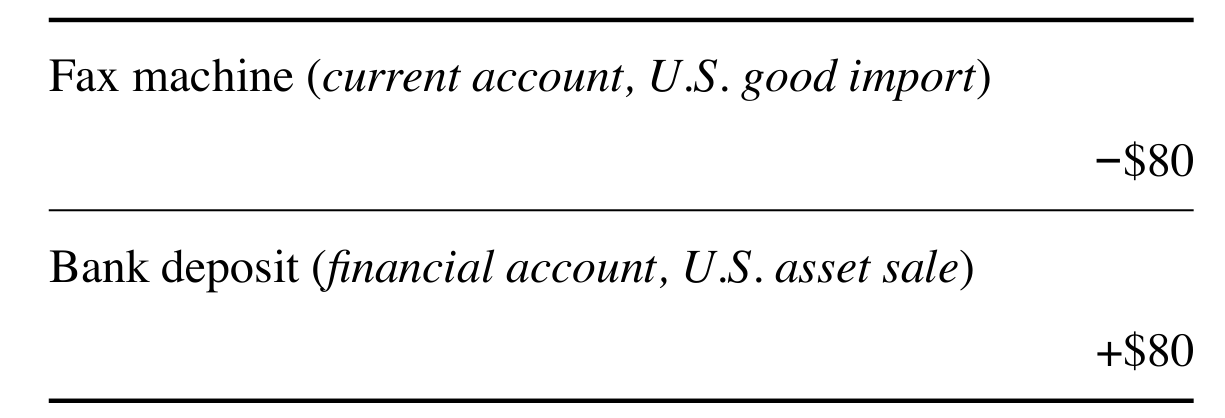
\includegraphics[width=0.85\textwidth]{num1.pdf}
	\label{fig:11}
\end{figure}
}


\frame{
\frametitle{Example (2): Invest in the Japanese stock market.}
\begin{figure}
	\centering
		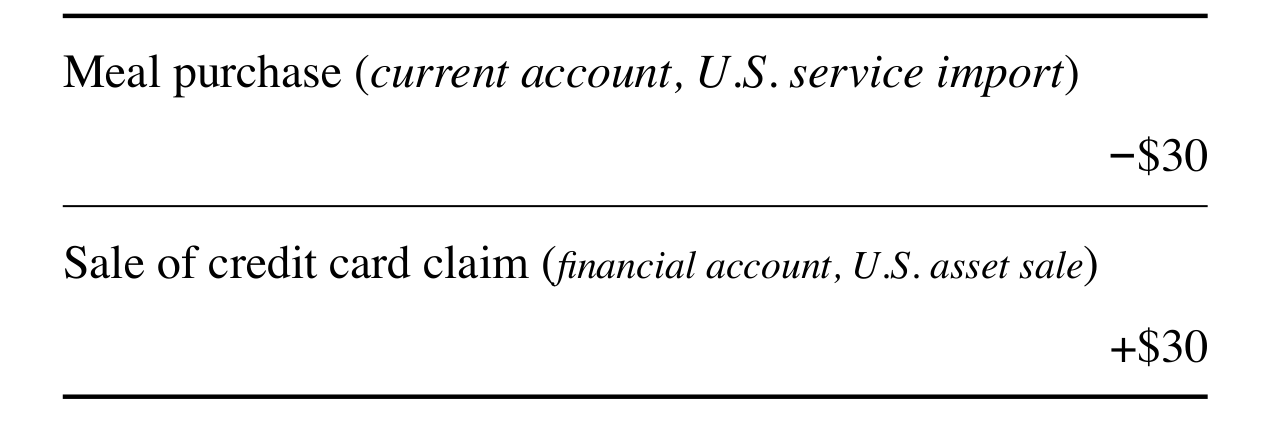
\includegraphics[width=0.85\textwidth]{num2.pdf}
	\label{fig:11}
\end{figure}
}


\frame{
\frametitle{Example (3): Forgiving Argentinian Debt.}
\begin{figure}
	\centering
		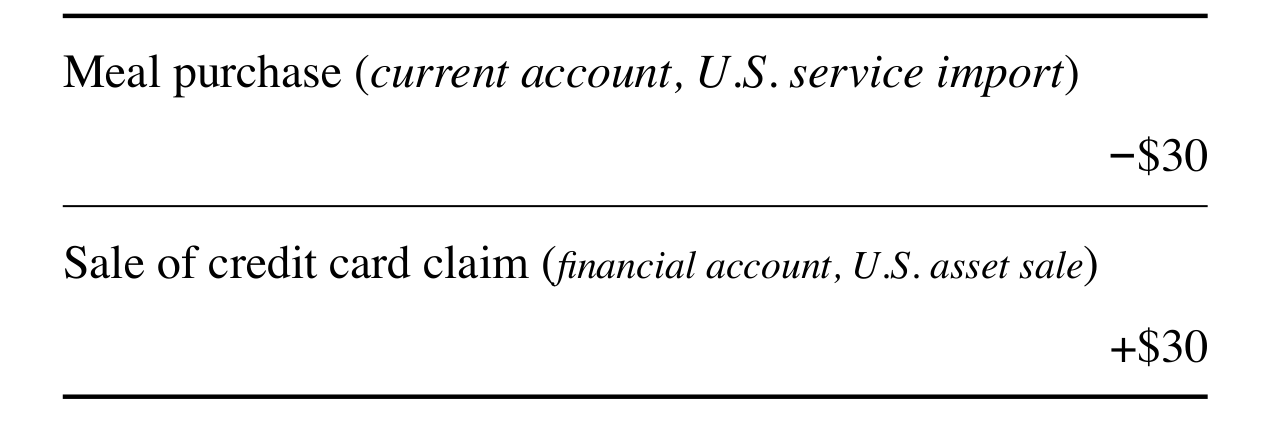
\includegraphics[width=0.85\textwidth]{num2.pdf}
	\label{fig:11}
\end{figure}
}



\frame{
\frametitle{U.S. Balance of Payments Accounts for 2006 (billions of dollars)}
\begin{figure}
	\centering
		\includegraphics[width=0.85\textwidth]{tab1.pdf}
	\label{fig:11}
\end{figure}
}


\frame{
\frametitle{U.S. Balance of Payments Accounts for 2006 (billions of dollars)}
\begin{figure}
	\centering
		\includegraphics[width=0.85\textwidth]{tab2.pdf}
	\label{fig:11}
\end{figure}
}



\frame{
\frametitle{Fig. 13-3: U.S. Gross Foreign Assets and Liabilities, 1976--2009}
\begin{figure}
	\centering
		\includegraphics[width=0.85\textwidth]{fig3new.pdf}
	\label{fig:11}
\end{figure}
}


\Section{Chapter 14. Exchange Rates and the Foreign Exchange Market: An Asset Approach}
\frame[plain]{% how to print
\frametitle{}
\begin{center}
\textcolor{blue}{\Huge{\textbf{Chapter 14: Exchange Rates and the Foreign Exchange Market: An Asset Approach
}}}
\end{center}
}


\Section{Chapter 14. Exchange Rates}
\frame{
\frametitle{Exchange Rates}
If you live in Denmark:
\begin{itemize}
\item \textbf{Direct}: The price of the foreign currency in terms
of DKK (e.g., $7.45$ DKK per Euro): $E_{DKK/EURO}$
\item \textit{Indirect} : The price of DKK in terms of the foreign currency (e.g., $0.13$ Euro per 1 DKK)
\end{itemize}
Exchange rate regimes:
\begin{itemize}
\item \textit{flexible}: Exchange rate is
determined by the market
\item \textit{fixed}: Exchange rate is
politically determined
\end{itemize}
}

\frame{
\frametitle{Figure: Fixed and Floating Exchange Rate }
\begin{figure}
	\centering
		\includegraphics[width=0.85\textwidth]{fixed.pdf}
	\label{fig:11}
\end{figure}
}

\frame{
\frametitle{Table 14-1: Exchange Rate Quotations}
\begin{figure}
	\centering
		\includegraphics[width=0.85\textwidth]{exrate.pdf}
	\label{fig:11}
\end{figure}
}

\frame{
\frametitle{Depreciation and Appreciation}
We are under \textbf{flexible exchange rates}:
\begin{enumerate}
\item \textbf{Depreciation} $E_{DKK/EURO} \Uparrow$ the Euro becomes more
expensive, i.e., DKK becomes less valuable.
\item \textbf{Appreciation} $E_{DKK/EURO} \Downarrow$ the Euro becomes less
expensive, i.e., DKK becomes more
valuable.
\end{enumerate}
}


\frame{
\frametitle{Devaluation and Revaluation}
We are under \textbf{fixed exchange rates}:
\begin{enumerate}
\item \textbf{Devaluation} $E_{DKK/EURO} \Uparrow$ the Euro becomes more
expensive, i.e., DKK becomes less valuable.
\item \textbf{Revaluation} $E_{DKK/EURO} \Downarrow$ the Euro becomes less
expensive, i.e., DKK becomes more
valuable.
\end{enumerate}
}


\Section{Chapter 14. The Foreign Exchange Market}

\frame{
\frametitle{The Foreign Exchange Market}
Four actors:
\begin{enumerate}
\item \textbf{Commercial banks and other depository institutions}: transactions involve buying/selling of deposits in different currencies for investment purposes.
\item \textbf{Non-bank financial institutions} may buy/sell foreign assets for investment.
\item \textbf{Non-financial businesses} conduct foreign currency transactions to buy/sell goods, services and assets
\item \textbf{Central banks} conduct official international reserves transactions
\end{enumerate}
ICT and the integration of markets imply that there is no significant \textit{arbitrage}(=buying at a low price and selling at a high price for a profit) between markets.
}

\frame{
\frametitle{When Exchange Rates Misbehave (1)}
\begin{itemize}
\item \textbf{Exchange rate crises} occur when a currency experiences a sudden decrease in value against another currency.
\begin{itemize}
\item Such crises are fairly common � 19 crises 1980-2002
\end{itemize}
\item Crises can have severe economic consequences.
\begin{itemize}
\item Government default
\item Financial and banking collapses
\item Severe contraction in output and decline in real wages
\end{itemize}
\item Politically embarrassing
\begin{itemize}
\item Countries experiencing crises often seek help from international development agencies, such as the International Monetary Fund (IMF).
\end{itemize}
\end{itemize}}

\frame[plain]{
\frametitle{When Exchange Rates Misbehave (2). Source: IMF, International Financial Statistics.
}
\begin{figure}
	\centering
		\includegraphics[width=0.85\textwidth]{exratemis.pdf}
	\label{fig:11}
\end{figure}
}

\frame[plain]{
\frametitle{Case Study: Argentina (2001)
}
\begin{figure}
	\centering
		\includegraphics[width=0.85\textwidth]{argentina.pdf}
	\label{fig:11}
\end{figure}
}

\frame{
\frametitle{Spot and Forward Rates}
\begin{itemize}
\item \textbf{Spot rates}: exchange rates for currency exchanges "on the spot", or when trading is executed in the present.
\item \textbf{Forward rates}:  may buy/sell foreign assets for investment.
\end{itemize}
Other methods:
\begin{enumerate}
\item Foreign exchange swaps
\item Futures contracts
\item Options contracts
\end{enumerate}
}


\frame{
\frametitle{Fig. 14-1: Dollar/Pound Spot and Forward Exchange Rates, 1981-�2009 }
\begin{figure}
	\centering
		\includegraphics[width=0.85\textwidth]{131new.pdf}
	\label{fig:11}
\end{figure}
}

\Section{Chapter 14. The Demand of Currency Deposits}

\frame{
\frametitle{The Demand of Currency Deposits (1)}
Factors that influence the return on assets determine the demand of those assets.
\begin{itemize}
\item \textbf{Rate of return:} the \% change in value that an asset offers during a time period
\item \textbf{Real rate of return:} inflation-adjusted rate of return
\item if inflation=0 $\Rightarrow$ rate of return=real rate of return
\end{itemize}
}


\frame{
\frametitle{The Demand of Currency Deposits (2)}
Example:
Should we invest in a Danish bond or an Euro bond?
\begin{itemize}
\item 1 DKK in DK bonds $\Rightarrow \left(1+R_{DKK,t}\right)$ DKK in a year
\item 1 DKK in Euro bonds: $\Rightarrow \left(\frac{1}{E_{DKK/EURO,t}}\right)\left(1+R_{EURO,t}\right)$
\item at time $t+1$: $\Rightarrow E^{e}_{DKK/EURO,
t+1}\left(\frac{1}{E_{DKK/EURO,t}}\right)\left(1+R_{EURO,t}\right)$
\item No arbitrage: the two returns have to be equal
\end{itemize}
}


\frame{
\frametitle{The Uncovered Interest Parity (1)}
We can rewrite the relation as:
\begin{center}
$\left(1+R_{DKK,t}\right)=E^{e}_{DKK/EURO,t+1}\left(\frac{1}{E_{DKK/EURO,t}}\right)\left(1+R_{EURO,t}\right)$
\end{center}
\begin{center}
$\Rightarrow$
\end{center}
\begin{center}
$\left(1+R_{DKK,t}\right)=\left(1+R_{EURO,t}\right)\left(\frac{E^{e}_{DKK/EURO,t+1}}{E_{DKK/EURO,t}}\right)$
\end{center}
Taking logs,
\begin{center}
$R_{DKK,t}\approx R_{EURO,t}+\left(\frac{E^{e}_{DKK/EURO,t+1}-E_{DKK/EURO,t}}{E_{DKK/EURO,t}}\right)$
\end{center}
}



\frame{
\frametitle{The Uncovered Interest Parity (2)}
In other words, arbitrage ensures
that the domestic interest rate
equals the foreign interest rate plus
the expected percentage
depreciation of the domestic
currency.
\begin{itemize}
\item $E^{e}_{DKK/EURO,t+1}=E_{DKK/EURO,t} \Rightarrow R_{DKK,t}=R_{EURO,t}$
\end{itemize}
}


\frame{
\frametitle{Table 14-3: Comparing Dollar Rates of Return on Dollar and Euro Deposits}
\begin{figure}
	\centering
		\includegraphics[width=0.90\textwidth]{133.pdf}
	\label{fig:11}
\end{figure}
}


\frame{
\frametitle{Equilibrium in the Foreign
Exchange Market}
The Equilibrium Exchange Rate
\begin{itemize}
\item Exchange rates always adjust to
maintain interest parity.
\item Assume that the DKK interest rate
$R_{DKK}$, the Euro interest rate $R_{EURO}$, and
the expected future DKK/EURO
exchange rate $E_{e}$, are all given
\end{itemize}
}

\frame{
\frametitle{Table 14-4: }
\begin{figure}
	\centering
		\includegraphics[width=0.90\textwidth]{135.pdf}
	\label{fig:11}
\end{figure}
}

\frame{
\frametitle{Fig. 14-3}
\begin{figure}
	\centering
		\includegraphics[width=0.90\textwidth]{fig133.pdf}
	\label{fig:11}
\end{figure}
}


\frame{
\frametitle{The Current Exchange Rate and the Expected Rate of Return on Dollar Deposits}
\begin{figure}
	\centering
		\includegraphics[width=0.90\textwidth]{fig134.pdf}
	\label{fig:11}
\end{figure}
}


\frame{
\frametitle{Fig. 14-4: Determination of the Equilibrium Dollar/Euro Exchange Rate}
\begin{figure}
	\centering
		\includegraphics[width=0.90\textwidth]{fig135.pdf}
	\label{fig:11}
\end{figure}
}


\frame{
\frametitle{Model of Foreign Exchange Markets }
The effects of changing interest rates: 
\begin{itemize}
\item an increase in the interest rate paid on deposits denominated in a particular currency will increase the rate of return on those deposits. 
\item this leads to an appreciation of the currency.
\end{itemize}
}

\frame{
\frametitle{Fig. 13-5: Effect of a Rise in the Dollar Interest Rate}
\begin{figure}
	\centering
		\includegraphics[width=0.90\textwidth]{fig136.pdf}
	\label{fig:11}
\end{figure}
}




\frame{
\frametitle{The Effect of an Expected Appreciation of the Euro}
\begin{figure}
	\centering
		\includegraphics[width=0.90\textwidth]{138.pdf}
	\label{fig:11}
\end{figure}
}

\frame{
\frametitle{Suggested Articles}
\begin{footnotesize}
\begin{thebibliography}{aaaaaaaaaaaaaaaaa}
\beamertemplatearticlebibitems
\bibitem[Jones]{jones1982}
Barro, R.
\newblock The Ricardian approach to budget deficits,
\newblock The Journal of Economic Perspectives 3 (2)., 1989
\beamertemplatearticlebibitems
\bibitem[Jones]{jones1982}
Burda, M.C., Severgnini, B.
\newblock Solow Residuals without Capital Stocks,
\newblock Journal of Development Economics, 2014
\beamertemplatearticlebibitems
\bibitem[Jonesa]{jonesa1982}
Giavazzi, F., Pagano, M.
\newblock Non-Keynesian Effects of Fiscal Policy Changes: International Evidence and the Swedish Experience
\newblock Swedish Economic Policy Review, 3, 67-103, 1996
\end{thebibliography}
\end{footnotesize}
}


\end{document}


